\documentclass[11pt,a4paper]{article}

% ------------------------------------------------------------------
% Packages
% ------------------------------------------------------------------
\usepackage[utf8]{inputenc}
\usepackage[T1]{fontenc}
\usepackage{lmodern}
\usepackage[margin=2.5cm]{geometry}
\usepackage{amsmath,amssymb,amsthm}
\usepackage{mathtools}
\usepackage{booktabs}
\usepackage{graphicx}
\usepackage{xcolor}
\usepackage{enumitem}
\usepackage{algorithm}
\usepackage{algpseudocode}
\usepackage{tikz}
\usetikzlibrary{arrows.meta,positioning,shapes.geometric,fit}
\usepackage[numbers,sort&compress]{natbib}
\usepackage[colorlinks=true,linkcolor=blue!60!black,citecolor=blue!60!black,urlcolor=blue!60!black]{hyperref}
\usepackage[nameinlink,capitalise]{cleveref}

% ------------------------------------------------------------------
% Theorem environments and macros
% ------------------------------------------------------------------
\newtheorem{definition}{Definition}
\newtheorem{assumption}{Assumption}
\newtheorem{proposition}{Proposition}

\newcommand{\E}{\mathbb{E}}
\newcommand{\Prob}{\mathbb{P}}
\newcommand{\R}{\mathbb{R}}
\newcommand{\KL}{\mathrm{KL}}

\title{A Hierarchical Adaptive Standard Gamble for Cross-Species Welfare Valuation\\
\large A Conceptual Proposal with a Synthetic Benchmark}

\author{Kai Yi Ji}
\date{}
\hypersetup{pdftitle={A Hierarchical Adaptive Standard Gamble for Cross-Species Welfare Valuation: A Conceptual Proposal with a Synthetic Benchmark},pdfauthor={Kai Yi Ji}}
% Generated by simulate.py.
\newcommand{\SimSeed}{20261125}
\newcommand{\SimN}{320}
\newcommand{\SimCohorts}{4}
\newcommand{\SimHistory}{36}
\newcommand{\SimBudget}{36}
\newcommand{\SimCalibration}{12}
\newcommand{\SimWidth}{0.20}
\newcommand{\SimDiscrepancy}{0.0021}
\newcommand{\SimResultRows}{%
Matched & Deterministic SG & 0.107 & +0.018 & 0.0 & 3 & 100.0 \\
 & Prob. bisection & 0.072 & +0.035 & 9.7 & 10 & 100.0 \\
 & Bayes (flat) & 0.072 & -0.040 & 99.7 & 36 & 9.1 \\
 & Two-stage HA-SG & 0.049 & -0.008 & 96.2 & 25 & 83.1 \\
\midrule
High lapses & Deterministic SG & 0.168 & +0.000 & 0.0 & 3 & 100.0 \\
 & Prob. bisection & 0.089 & +0.034 & 10.6 & 10 & 99.7 \\
 & Bayes (flat) & 0.132 & +0.013 & 82.2 & 36 & 21.9 \\
 & Two-stage HA-SG & 0.058 & +0.005 & 89.1 & 25 & 90.3 \\
\midrule
Population shift & Deterministic SG & 0.136 & -0.052 & 0.0 & 3 & 100.0 \\
 & Prob. bisection & 0.119 & -0.071 & 8.4 & 9 & 100.0 \\
 & Bayes (flat) & 0.092 & -0.047 & 98.4 & 36 & 6.2 \\
 & Two-stage HA-SG & 0.061 & +0.013 & 96.2 & 36 & 12.2 \\
\midrule
Task shift & Deterministic SG & 0.135 & +0.095 & 0.0 & 3 & 100.0 \\
 & Prob. bisection & 0.123 & +0.106 & 3.1 & 8 & 100.0 \\
 & Bayes (flat) & 0.059 & +0.018 & 98.1 & 36 & 20.3 \\
 & Two-stage HA-SG & 0.072 & +0.055 & 73.1 & 23 & 96.9 \\
}
\newcommand{\SimCalibrationRows}{%
Matched & 0.033 \\
High lapses & 0.041 \\
Population shift & 0.066 \\
Task shift & 0.074 \\
}


\begin{document}

\maketitle

\begin{abstract}
The Standard Gamble (SG) estimates the value of a health state from the probability at which a respondent is indifferent between that state and a gamble. Inconsistent responses can derail deterministic bisection, and probability weighting can affect the estimated value even when responses are consistent. We propose a hierarchical adaptive Standard Gamble (HA-SG) that uses a Bayesian choice model to learn patterns from previous respondents and choose an informative first offer. The model can account for geographic differences among human samples and borrow information across species where tasks support it. Later offers adapt to the individual's responses. A behavioural Standard Gamble for non-human animals uses experienced probabilities and welfare-acceptable outcomes. A two-stage design first estimates probability weighting in a reward task and then uses that estimate to infer state utility, conditional on the weighting function carrying over between tasks. The resulting utilities are relative to the chosen anchors.
 A synthetic Monte Carlo benchmark compares four elicitation methods. Two-stage HA-SG has the lowest observed root mean squared error in three of the four scenarios. When weighting differs between tasks, single-stage Bayesian elicitation has lower error and higher coverage at the 36-trial budget.
\end{abstract}

\noindent\textbf{Keywords:} Standard Gamble; health-state utility; adaptive design optimisation; probabilistic bisection; Bayesian inference; risk-sensitive foraging; comparative cognition; animal welfare

% ==================================================================
\section{Introduction}
\label{sec:intro}
% ==================================================================

Quantifying how good or bad it is to live in a given state is central to economic evaluation in health care. Quality-adjusted life years (QALYs) require health-state utilities on a scale anchored at full health (1) and death (0), and the Standard Gamble (SG) is the method most directly grounded in expected utility theory for obtaining them \citep{vonneumann1944,torrance1986,drummond2015,brazier2017}. In an SG task, a respondent compares living with certainty in a health state $h$ against a gamble that yields full health with probability $p$ and immediate death with probability $1-p$. The probability $p^\ast$ at which the respondent is indifferent is interpreted as the utility of $h$.

In practice, $p^\ast$ is rarely asked for directly. Instead, it is located through a sequence of binary choices---``ping-pong'', titration or bisection procedures---that progressively narrow the interval in which indifference lies \citep{lenert1998}. Viewed computationally, this is a binary search. Binary search is extremely efficient when every answer is correct, but SG responses are not: respondents make errors, exhibit reference dependence, and distort probabilities \citep{kahneman1979,tversky1992,bleichrodt2002}. A single early inconsistent response can permanently exclude the true indifference point from the search interval. Moreover, even a perfectly consistent respondent's $p^\ast$ reflects not only the value of $h$ but also their attitude towards risk, so the elicited ``utility'' is a composite quantity \citep{bleichrodt2001}.

The proposal has three parts.
\begin{enumerate}[leftmargin=*]
  \item \textbf{Algorithmic.} We recast iterative SG as noisy search and propose using patterns learned from earlier respondents to choose the first offer, then adapting to the individual's answers. The approach builds on probabilistic bisection \citep{horstein1963,burnashev1974,waeber2013} and hierarchical adaptive design \citep{myung2013,cavagnaro2013,kim2014}.
  \item \textbf{Conceptual.} We extend the SG beyond humans by defining a \emph{behavioural Standard Gamble} in which hypothetical descriptions are replaced by experienced, safe choices, drawing on the literature on risk-sensitive foraging and comparative decision-making \citep{caraco1980,kacelnik1996,heilbronner2008,stauffer2015}.
  \item \textbf{Methodological.} We formalise the distinction between \emph{risk attitude} and \emph{state utility}, show that a single indifference point cannot identify both, and give conditions under which a two-stage calibration design separates them.
\end{enumerate}

The contribution is the integration of these methods into a behavioural Standard Gamble. Corrections for probability weighting and hierarchical estimation of human health-state utilities already exist. The proposed adaptation combines separate reward calibration, adaptive offers and welfare-acceptable anchors to estimate how an animal values a specific condition.

Risk preferences vary across species and, in humans, both within and across countries \citep{heilbronner2008,rosati2011,hayden2007,falk2018}. These differences motivate a model that allows for individual variation while pooling information from comparable tasks and populations.

% ==================================================================
\section{Background}
\label{sec:background}
% ==================================================================

\subsection{The Standard Gamble}

\paragraph{The indifference point.} The indifference point $p^\ast$ is the chance of the better outcome at which a person values the gamble and the certain option equally. For example, suppose someone prefers the certain health state when the gamble offers a $60\%$ chance of full health, prefers the gamble at $70\%$, and values the two options equally at $65\%$. Their indifference point is $p^\ast=0.65$. The $65\%$ refers to the chance of full health if they take the gamble. Under the symmetric noisy-choice model below, the person is predicted to choose each option with probability $50\%$ at that offer.

\paragraph{From indifference to utility.}

Let $\mathrm{FH}$ denote full health, $\mathrm{D}$ death and $h$ an intermediate health state. Under expected utility (EU) with the normalisation $U(\mathrm{FH})=1$, $U(\mathrm{D})=0$, indifference between $h$ for certain and the lottery $(\mathrm{FH},p;\mathrm{D},1-p)$ implies
\begin{equation}
  U(h) = p^\ast U(\mathrm{FH}) + (1-p^\ast)U(\mathrm{D}) = p^\ast.
  \label{eq:sg-eu}
\end{equation}
The SG is therefore the ``gold standard'' in the sense of being normatively derived from EU \citep{torrance1986}. Empirically, however, SG utilities are systematically higher than time trade-off utilities, a gap that has been attributed to probability weighting and loss aversion \citep{bleichrodt2002}. If choices follow rank-dependent utility or prospect theory with a probability weighting function $w(\cdot)$, then indifference implies
\begin{equation}
  U(h) = w(p^\ast),
  \label{eq:sg-rdu}
\end{equation}
The indifference point is therefore an offered probability, and the choice model determines how to translate it into a utility. Reporting $p^\ast$ as $U(h)$ is biased whenever $w(p^\ast)\neq p^\ast$ \citep{bleichrodt2001}. Common parametric forms include the one-parameter \citet{prelec1998} function $w(p)=\exp(-(-\ln p)^{\alpha})$ and the \citet{tversky1992} form.

\citet{wakker1995} proposed a rank-dependent correction for human SG. \citet{lipman2019} empirically applied prospect-theory corrections accounting for probability weighting, loss aversion and nonlinear utility of life duration.

\subsection{Iterative elicitation as binary search}

Let $p\in[0,1]$ be the gamble probability offered at a given step. A deterministic respondent with indifference point $p^\ast$ prefers the gamble iff $p>p^\ast$. Bisection maintains an interval $[a,b]\ni p^\ast$ and offers $p=(a+b)/2$, halving the interval at each step; after $n$ questions the uncertainty is $2^{-n}$. Different search procedures (bisection, ping-pong, titration) are known to yield different utilities \citep{lenert1998}, which already signals that the response process is not deterministic.

With noisy responses---each answer wrong with probability $\varepsilon>0$---deterministic bisection is inconsistent: an early error removes $p^\ast$ from the interval forever. The \emph{probabilistic bisection algorithm} (PBA) instead maintains a posterior density over $p^\ast$ and queries its median, updating multiplicatively by the likelihood of each response \citep{horstein1963,burnashev1974}. PBA converges under fairly general conditions \citep{waeber2013}, and noisy binary search more broadly has well-studied complexity guarantees \citep{karp2007}.

\subsection{Adaptive design in psychophysics and decision science}

Psychophysics has long used Bayesian adaptive procedures to estimate thresholds of psychometric functions, e.g.\ QUEST and the $\Psi$ method \citep{watson1983,kontsevich1999}. Adaptive design optimisation (ADO) generalises this idea by selecting each stimulus to maximise expected information about model parameters \citep{chaloner1995,myung2013}. ADO has been applied to risky choice to discriminate between models and estimate risk parameters \citep{cavagnaro2013,toubia2013}. Here, the same design principle is used to select offers that inform the estimate of state utility.

\citet{kim2014} used data from earlier participants to inform adaptive testing of new participants. In health-state valuation, \citet{lipmanpachur2025} used a hierarchical Bayesian choice model to estimate human SG and time trade-off utilities from trials presented in random order. The proposed design uses the model to select each offer as well as to estimate utility.

\subsection{Risk preferences across species}

Behavioural ecology studies \emph{risk-sensitive foraging}: animals choosing between a constant food option and a variable one with equal or differing means \citep{caraco1980,stephens1986,kacelnik1996}. Risk attitudes vary with energy budget, with whether variance is in amount or in delay, and across taxa \citep{kacelnik1996}. Among primates, chimpanzees have been found more risk-prone than bonobos in a food-gamble task \citep{heilbronner2008}, the two species distinguish risk from ambiguity \citep{rosati2011}, and rhesus macaques show risk-seeking that covaries with temporal discounting \citep{hayden2007}. Economic choices of macaques reveal non-linear probability weighting broadly resembling that of humans \citep{stauffer2015}.

A critical difference from human SG is that animals typically learn outcome probabilities through experience rather than description. Human research shows that decisions from experience can systematically differ from decisions from description, notably in the weighting of rare events \citep{hertwig2004}. Animal titration procedures, such as the adjusting-delay procedure \citep{mazur1987}, are already behavioural analogues of iterative search.

\subsection{Choice-based measures of animal welfare}

Animal welfare science uses preference and motivation tests---what an animal will choose and how hard it will work for it---as evidence about its subjective states \citep{dawkins1990,kirkden2003}, alongside cognitive-bias tests interpreting ambiguous-cue responses as indicators of affective state \citep{harding2004,mendl2010}. These literatures provide both the experimental paradigms and the caution needed for any attempt to elicit ``utility'' from animal choices.

% ==================================================================
\section{A Noisy-Choice Model of the Standard Gamble}
\label{sec:model}
% ==================================================================

We model each subject $i$ (human or animal) using contextual information $x_i$, which can include species, recruitment location for human samples, and the task and outcomes on offer.

\begin{definition}[SG choice model]
\label{def:choice}
On trial $t$, subject $i$ is offered gamble probability $p_t$. Let $Y_{it}=1$ if the gamble is chosen. Then
\begin{equation}
  \Prob(Y_{it}=1 \mid p_t,\theta_i)
  = \varepsilon_i + (1-2\varepsilon_i)\,
    F\!\left(\lambda_i\big[w_{\alpha_i}(p_t) - u_i\big]\right),
  \label{eq:choice}
\end{equation}
where $u_i\in(0,1)$ is the target state utility, $w_{\alpha_i}$ is a probability weighting function with curvature $\alpha_i$, $\lambda_i>0$ is choice sensitivity (inverse noise), $\varepsilon_i\in[0,\tfrac12)$ is a lapse rate, and $F$ is a sigmoid (logistic or standard normal CDF). We write $\theta_i=(u_i,\alpha_i,\lambda_i,\varepsilon_i)$.
\end{definition}

This is a standard random-utility formulation \citep{luce1959,hey1994} adapted to the SG. At $p_i^\ast$, the difference $w_{\alpha_i}(p_i^\ast)-u_i$ is zero. Since $F(0)=1/2$ for the logistic and standard normal links, \cref{eq:choice} gives a gamble-choice probability of $1/2$ even with symmetric lapses. The model nests the classical case: as $\lambda_i\to\infty$, $\varepsilon_i\to 0$ and $\alpha_i\to 1$ (so $w(p)=p$), choices away from $p_i^\ast=u_i$ become deterministic.

\paragraph{Learning from previous respondents.}
Let $\mathcal H$ be earlier choice data and $\Phi$ the population parameters. For a new subject, the predictive prior is
\begin{equation}
  \pi_0(\theta_i\mid x_i,\mathcal H)
  = \int \pi(\theta_i\mid x_i,\Phi)\,\pi(\Phi\mid\mathcal H)\,d\Phi.
  \label{eq:learned-prior}
\end{equation}
Learning $\pi(\Phi\mid\mathcal H)$ is the machine-learning step that informs the first offer. The hierarchy can learn variation between human recruitment locations while partially pooling local estimates towards a broader human distribution. Geography indicates the context in which responses were collected. Differences may reflect recruitment, task wording or other local conditions as well as preferences. Across species, comparable tasks can inform shared aspects of choice, such as consistency or probability weighting, while allowing species-specific distributions. Utilities tied to different outcomes and anchors remain task-specific. A new or sparsely sampled setting can draw on a broader prior with greater uncertainty.

\paragraph{Target and nuisance parameters.}
The quantity of interest is $u_i$ (and, at group level, its distribution). The parameters $(\alpha_i,\lambda_i,\varepsilon_i)$ are nuisance parameters that must nonetheless be learned, because they determine how informative each choice is about $u_i$.

% ==================================================================
\section{Bayesian Adaptive Search}
\label{sec:algorithm}
% ==================================================================

The learned choice model guides which question to ask next.

\begin{enumerate}[leftmargin=*]
  \item \textbf{Belief state.} Start with the learned prior in \cref{eq:learned-prior}. After each answer, update the distribution of $\theta_i$ using the subject's own responses.
  \item \textbf{Design selection.} The next offer $p_{t+1}$ is chosen to maximise expected information gain about the \emph{target} $u_i$, marginalising over nuisance parameters:
  \begin{equation}
    p_{t+1} = \arg\max_{p\in\mathcal{P}}\;
    \E_{Y\sim \Prob(\cdot\mid p,\mathcal{D})}
    \Big[\KL\big(\pi(u_i\mid \mathcal{D},p,Y)\,\big\|\,\pi(u_i\mid\mathcal{D})\big)\Big].
    \label{eq:eig}
  \end{equation}
  Here $\mathcal D$ includes $x_i$, the earlier data $\mathcal H$, and any answers from subject $i$. For the first offer, there are no individual answers yet, so the calculation uses the learned prior.

  Classification trees can score a split by either Shannon information gain or Gini impurity reduction. In a forest, \emph{Gini importance} aggregates the weighted Gini reductions from splits that use a given feature \citep{louppe2013}. The analogue for offer selection is the expected Gini impurity reduction from a single response.

  To apply this criterion, partition the range of $u_i$ into fixed intervals and let $q_j$ be the current posterior probability of interval $j$. The Gini impurity is $G(q)=1-\sum_j q_j^2$. For a candidate offer $p$, compute the posterior interval probabilities $q^{(y)}$ after each possible response $y$. Score the offer by
  \[
    G(q)-\sum_y \Prob(Y=y\mid p,\mathcal{D})\,G(q^{(y)}).
  \]
  This score measures how well the offer distinguishes the chosen utility intervals and can depend on their boundaries. Expected posterior variance reduction instead scores offers on the original utility scale and matches a squared-error estimation objective. A cost for additional trials can also be incorporated for welfare reasons.
  \item \textbf{Stopping rule.} Stop when the posterior credible interval for $u_i$ is narrower than a tolerance $\delta$, or a maximum number of trials $T_{\max}$ is reached.
\end{enumerate}

\begin{algorithm}[t]
\caption{Hierarchical adaptive Standard Gamble (HA-SG)}
\label{alg:hasg}
\begin{algorithmic}[1]
\Require Earlier data $\mathcal H$, context $x_i$, offers $\mathcal{P}\subset(0,1)$, tolerance $\delta$, budget $T_{\max}$
\State Initialise $\pi_0(\theta_i)$ from the learned prior in \cref{eq:learned-prior}
\For{$t = 0,1,\dots,T_{\max}-1$}
  \State Choose $p_{t+1}$ by maximising expected information gain on $u_i$ (\cref{eq:eig})
  \State Present choice; observe $Y_{i,t+1}\in\{0,1\}$
  \State Update $\pi_{t+1}(\theta_i) \propto \pi_t(\theta_i)\,\Prob(Y_{i,t+1}\mid p_{t+1},\theta_i)$
  \If{width of 95\% credible interval of $u_i$ $< \delta$}
    \State \textbf{break}
  \EndIf
\EndFor
\State Update the population model with subject $i$'s data for future subjects
\State \Return posterior of $u_i$ (and of $\alpha_i,\lambda_i,\varepsilon_i$)
\end{algorithmic}
\end{algorithm}

\paragraph{Choosing where to start.}
An intuitive starting rule is to compute the distribution of $p_i^\ast=w_{\alpha_i}^{-1}(u_i)$ under the learned prior and offer the candidate probability nearest its median. If that median is $0.65$, the model puts half of the predicted indifference points on each side of $0.65$ for a continuous prior. In noiseless bisection on the threshold, the first answer at this offer would distinguish between two equally probable ranges. A higher predicted threshold can arise from stronger probability underweighting or from a higher state utility. The information-gain rule in \cref{eq:eig} selects the first offer directly for learning $u_i$ and can choose a different value when utility and probability weighting are both uncertain. In either case, the full set of candidate offers remains available as the subject answers (\cref{fig:starting-offer}).

\begin{figure}[htbp]
\centering
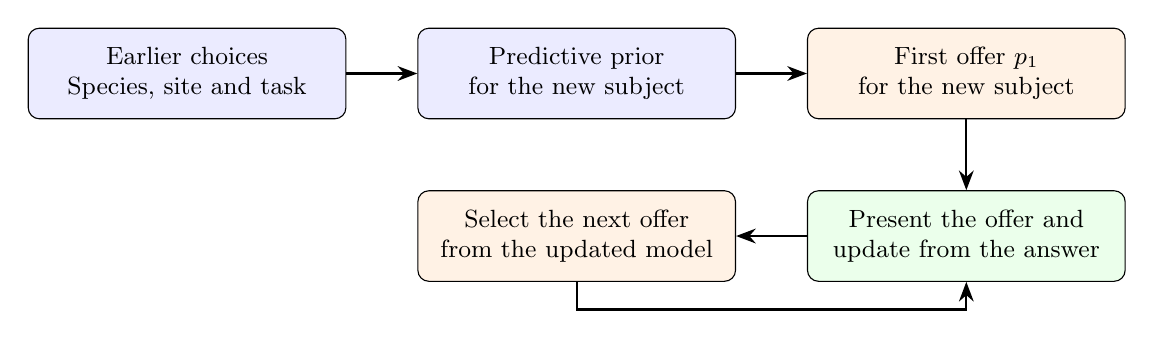
\begin{tikzpicture}[
  node distance=0.9cm,
  box/.style={draw, rounded corners, align=center, text width=3.8cm, minimum height=1.15cm, font=\small},
  arr/.style={-{Stealth[length=2.5mm]}, thick}
]
\node[box, fill=blue!8] (data) {Earlier choices\\Species, site and task};
\node[box, fill=blue!8, right=of data] (prior) {Predictive prior\\for the new subject};
\node[box, fill=orange!10, right=of prior] (offer) {First offer $p_1$\\for the new subject};
\node[box, fill=green!8, below=of offer] (update) {Present the offer and\\update from the answer};
\node[box, fill=orange!10, left=of update] (next) {Select the next offer\\from the updated model};
\draw[arr] (data) -- (prior);
\draw[arr] (prior) -- (offer);
\draw[arr] (offer) -- (update);
\draw[arr] (update) -- (next);
\draw[arr] (next.south) -- ++(0,-0.35) -| (update.south);
\end{tikzpicture}
\caption{Earlier choice data inform the first gamble offer. Each answer then updates the model for the individual and guides the next offer.}
\label{fig:starting-offer}
\end{figure}

\paragraph{Relation to classical methods.}
With $w(p)=p$, a step-function response model, and a known symmetric error rate $\varepsilon<1/2$, the posterior median of $u_i$ maximises expected information gain whenever that offer is available. Querying this median gives probabilistic bisection \citep{waeber2013}. With $\varepsilon=0$ and a uniform prior on the initial interval, the median is the midpoint of the remaining interval, giving deterministic bisection.

\paragraph{Implementation.}
For a low-dimensional $\theta_i$, the posterior can be maintained on a grid or with sequential Monte Carlo, and \cref{eq:eig} evaluated over a discrete $\mathcal{P}$ in real time. Group-level updates can be performed offline with Markov chain Monte Carlo between subjects. Amortised or neural approaches to design selection are a possible extension but are not required.

% ==================================================================
\section{A Behavioural Standard Gamble for Non-Human Animals}
\label{sec:behavioural}
% ==================================================================

\subsection{Why the human SG cannot be transferred directly}

The human SG relies on (i) understanding described probabilities, (ii) imagining hypothetical health states, and (iii) anchoring on death. None of these is available, or ethically acceptable, for non-human animals. A behavioural adaptation must therefore use:
\begin{itemize}[leftmargin=*]
  \item \textbf{Experienced probabilities:} distinct cues (e.g.\ coloured levers, locations) are associated through training with known reward probabilities;
  \item \textbf{Safe, bounded outcomes:} outcomes are rewards or access to environments within welfare-acceptable bounds, never harm or death;
  \item \textbf{Observable choice:} preference is inferred from repeated choices, which are naturally modelled by \cref{eq:choice}.
\end{itemize}

\subsection{Bounded anchors}

In place of $\mathrm{FH}$ and $\mathrm{D}$ we use a best available state $B$ and a worst acceptable state $W$ from a defined set of conditions (e.g.\ enriched versus barren but welfare-compliant housing for a fixed period, or a preferred versus non-preferred food). Indifference between a state $A$ for certain and the lottery $(B,p;W,1-p)$ yields, under the choice model,
\begin{equation}
  \tilde u(A) \coloneqq \frac{U(A)-U(W)}{U(B)-U(W)} = w(p^\ast).
  \label{eq:bounded}
\end{equation}
This gives a utility relative to locally chosen anchors. A cross-species comparison requires evidence or assumptions that link the meaning of the scales (\cref{sec:discussion}).

\subsection{Worked example with a rat choosing enrichment}
\label{sec:rat-example}

Suppose a rat prefers brief access to a familiar play area with a tunnel and nesting material ($B$) over access to the same area with nesting material alone ($A$), and prefers either over access to the baseline area with its usual bedding ($W$). These rankings would first be checked with choices between the certain options. All three outcomes involve the same access time and leave the rat's normal housing and care in place.

On one trial, one cue offers $A$ for certain. The other offers a $70\%$ chance of $B$ and a $30\%$ chance of $W$. The rat learns these associations through experience. By varying the probability across trials, the procedure estimates the chance of $B$ at which the rat is equally likely to choose the gamble or take $A$ for certain. Suppose this indifference point is $0.70$. With linear weighting, $A$ has a relative utility of $0.70$ between $W$ and $B$. If a separate reward task with food pellets yields the illustrative weighting function $w(p)=p^2$, and that function carries over to the play-area task, the same indifference point implies a utility of $0.49$ (\cref{fig:weighting}). The estimate describes the value of this enrichment option between the two specified conditions.

% ==================================================================
\section{Separating Risk Attitude from State Utility}
\label{sec:separation}
% ==================================================================

An animal's willingness to accept an uncertain food reward does not, by itself, establish how good its current state is. The following makes this precise.

\begin{proposition}[Non-identification from a single gamble type]
\label{prop:nonid}
An indifference point $p^\ast$ from choices between $A$ for certain and $(B,p;W,1-p)$ cannot identify $\tilde u(A)$ when the strictly increasing weighting function $w$ is unknown. For any strictly increasing $g:[0,1]\to[0,1]$ with $g(0)=0$ and $g(1)=1$, the pair $(w',\tilde u')=(g\circ w,\;g(\tilde u))$ gives the same indifference point.
\end{proposition}

\noindent\emph{Sketch.} Applying $g$ to both sides of $w(p^\ast)=\tilde u$ preserves the equality and the ordering of offers relative to $p^\ast$. Identification from the shape of the full response curve would require additional assumptions about the weighting function and the response model. \qed

\smallskip
A high indifference probability can reflect a high value of $A$ under linear weighting or a lower value of $A$ when the gamble's success probability is underweighted (\cref{fig:weighting}). Probability weighting has also been proposed as one explanation for differences between SG and time trade-off utilities \citep{bleichrodt2002}.

\begin{figure}[htbp]
\centering
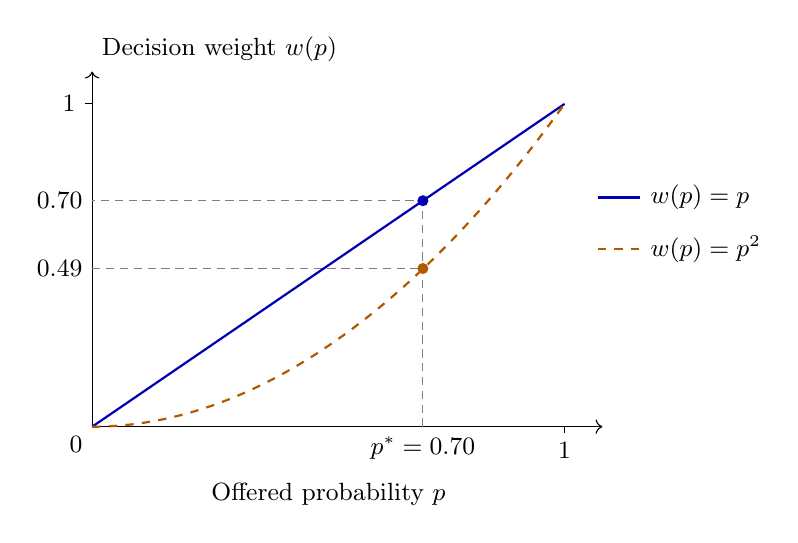
\begin{tikzpicture}[x=6cm,y=4.1cm, font=\small]
  \draw[->] (0,0) -- (1.08,0);
  \draw[->] (0,0) -- (0,1.10) node[above right] {Decision weight $w(p)$};
  \node[below=17pt] at (0.5,0) {Offered probability $p$};
  \node[below left] at (0,0) {$0$};
  \draw (0,1) -- (-0.015,1) node[left] {$1$};
  \draw (1,0) -- (1,-0.02) node[below] {$1$};
  \draw[densely dashed, gray] (0.70,0) -- (0.70,0.70)
    -- (0,0.70) node[left, black] {$0.70$};
  \draw[densely dashed, gray] (0,0.49) node[left, black] {$0.49$}
    -- (0.70,0.49);
  \draw[thick, blue!70!black] (0,0) -- (1,1);
  \draw[thick, orange!70!black, dashed] (0,0) parabola (1,1);
  \fill[blue!70!black] (0.70,0.70) circle[radius=2pt];
  \fill[orange!70!black] (0.70,0.49) circle[radius=2pt];
  \node[below] at (0.70,0) {$p^\ast=0.70$};
  \draw[thick, blue!70!black] (1.07,0.71) -- (1.16,0.71)
    node[right, black] {$w(p)=p$};
  \draw[thick, orange!70!black, dashed] (1.07,0.55) -- (1.16,0.55)
    node[right, black] {$w(p)=p^2$};
\end{tikzpicture}
\caption{Illustration of why the indifference probability alone cannot identify state utility. At the same observed $p^\ast=0.70$, linear weighting implies $\tilde u(A)=0.70$, while quadratic weighting implies $\tilde u(A)=0.49$.}
\label{fig:weighting}
\end{figure}

\subsection{Two-stage calibration design}

The calibration design aims to identify the probability weighting function in a separate reward task and use it to interpret the state-gamble indifference point.

\begin{assumption}[Domain-general probability weighting]
\label{ass:domain}
Within a subject, the same weighting function $w_{\alpha_i}$ governs choices over (i) reward lotteries and (ii) state lotteries.
\end{assumption}

\begin{description}[leftmargin=*]
  \item[Stage A (risk calibration).] Use choices between a certain reward $x$ and lotteries over reward amounts. Vary probabilities and amounts, including the lower outcome where feasible. Separating reward value $v$ from probability weighting $w_{\alpha_i}$ depends on the offers and the assumptions used to fit both functions \citep{wakker2008,stauffer2015}.
  \item[Stage B (state valuation).] Present state lotteries $(A)$ versus $(B,p;W,1-p)$ and estimate $\tilde u_i(A)$ using \cref{eq:choice}, with the posterior for $\alpha_i$ from Stage A as the prior.
\end{description}

\begin{proposition}[Identification under calibration]
\label{prop:id}
Under \cref{ass:domain}, if Stage A identifies $w_{\alpha_i}$ and Stage B identifies an indifference point $p^\ast_i$, then $\tilde u_i(A)=w_{\alpha_i}(p^\ast_i)$.
\end{proposition}

Comparing weighting estimates across reward domains can probe the plausibility of \cref{ass:domain}. Even within one domain, weighting can be sensitive to the task. In rhesus macaques, changing the sequence of reward choices altered the estimated shape of the weighting function \citep{ferraritoniolo2019}. In \cref{fig:overview}, the adaptive design targets reward valuation and probability weighting in Stage A, then state utility in Stage B.

\begin{figure}[t]
\centering
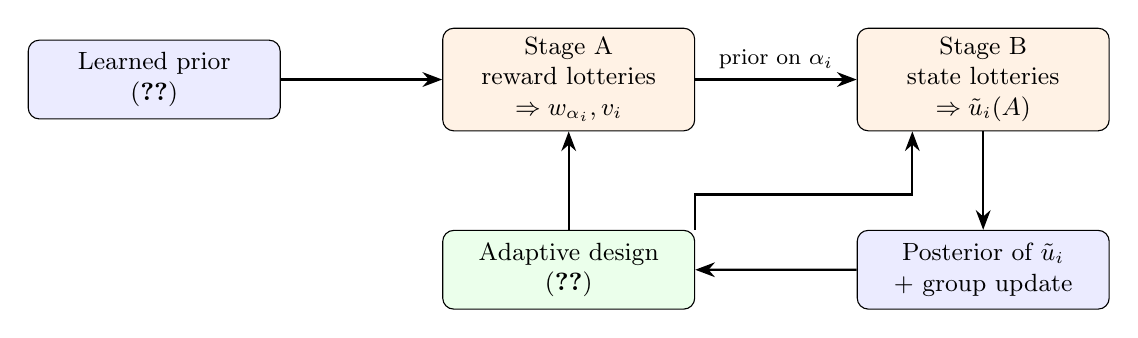
\begin{tikzpicture}[
  node distance=1.25cm and 2.05cm,
  box/.style={draw, rounded corners, align=center, minimum width=3.2cm, minimum height=1cm, font=\small},
  arr/.style={-{Stealth[length=2.5mm]}, thick}
]
\node[box, fill=blue!8] (prior) {Learned prior\\(\cref{eq:learned-prior})};
\node[box, fill=orange!10, right=of prior] (stageA) {Stage A\\reward lotteries\\$\Rightarrow w_{\alpha_i}, v_i$};
\node[box, fill=orange!10, right=of stageA] (stageB) {Stage B\\state lotteries\\$\Rightarrow \tilde u_i(A)$};
\node[box, fill=green!8, below=of stageA] (ado) {Adaptive design\\(\cref{eq:eig})};
\node[box, fill=blue!8, below=of stageB] (post) {Posterior of $\tilde u_i$\\$+$ group update};
\draw[arr] (prior) -- (stageA);
\draw[arr] (stageA) -- node[above, font=\footnotesize]{prior on $\alpha_i$} (stageB);
\draw[arr] (ado) -- (stageA);
\draw[arr] (ado.north east) -- ++(0,0.45) -| ([xshift=-9mm]stageB.south);
\draw[arr] (stageB) -- (post);
\draw[arr] (post.west) -- (ado.east);
\end{tikzpicture}
\caption{Proposed two-stage behavioural Standard Gamble. Stage A estimates how the subject weights probabilities. Stage B uses that estimate to infer state utility relative to welfare-acceptable anchors. The adaptive design guides offer selection in both stages.}
\label{fig:overview}
\end{figure}

\subsection{Sensitivity to probability weighting across tasks}
\label{sec:transfer-sensitivity}

Let $w_R$ be the weighting function in the reward task and $w_S$ the function in the state task. For a given state-gamble indifference point $p^\ast$, calibration under exact transfer assigns utility $w_R(p^\ast)$, while the state-choice model implies $\tilde u(A)=w_S(p^\ast)$. If the two decision weights differ by at most $\Delta$ at this offer, the resulting utility is bounded by
\begin{equation}
  \tilde u(A)\in
  \bigl[\max\{0,w_R(p^\ast)-\Delta\},\,
        \min\{1,w_R(p^\ast)+\Delta\}\bigr].
  \label{eq:transfer-bound}
\end{equation}
In the rat example, if $w_R(0.70)=0.49$ and the state-task weight could differ by up to $0.10$, the compatible utilities range from $0.39$ to $0.59$. The assumed $\Delta$ measures the allowed difference between tasks. Sampling uncertainty in $p^\ast$ and $w_R$ can be propagated separately by evaluating the bounds over posterior draws, estimating $p^\ast$ from the state choices without imposing exact transfer.

% ==================================================================
\section{Synthetic Monte Carlo Experiment}
\label{sec:simulation}

The experiment tests whether the four procedures recover a known utility under a common response budget. In each scenario, \SimN{} held-out synthetic subjects were evaluated across \SimCohorts{} independently generated cohorts. Each cohort had a separate training history of \SimHistory{} subjects, with 24 reward and 24 state choices per historical subject. All four methods faced the same held-out subjects and used common random draws for corresponding state responses. Each method had up to \SimBudget{} responses for a new subject. Two-stage HA-SG used \SimCalibration{} of these for reward calibration, leaving 24 for the state task.

\subsection{Generative model and fitted methods}

Synthetic state choices followed \cref{eq:choice}, using a logistic link, slope 16, and $w_S(p)=p^{\gamma_S}$. Reward choices used $v(x)=x^\rho$ and $w_R(p)=p^{\gamma_R}$. Reward lotteries varied both endpoints, including nonzero lower outcomes. The historical and matched populations had utility and weighting exponents generated around means of $0.63$ and $1.20$, respectively. The scenarios were:
\begin{itemize}[leftmargin=*]
  \item \textbf{Matched.} The test population follows the historical distribution, with lapse probability floor $0.04$ and $\gamma_S=\gamma_R$.
  \item \textbf{High lapses.} The test lapse floor rises to $0.16$. The Bayesian fits retain their working value of $0.04$.
  \item \textbf{Population shift.} The test means change to $0.36$ for utility and $0.85$ for the weighting exponent. The historical model is fit to the original population.
  \item \textbf{Task shift.} The state exponent is $1.35\gamma_R$, while the two-stage fit assumes that the same weighting function governs both tasks.
\end{itemize}

Deterministic SG bisected the current bracket and reported its midpoint. Probabilistic bisection used a uniform threshold prior and a working symmetric error probability of $0.12$, offering the candidate closest to the posterior median. Both bisection methods reported the estimated threshold as the conventional SG utility. The Bayesian single-stage method used a uniform grid prior over utility and the state weighting exponent. Two-stage HA-SG learned a prior from earlier subjects, selected reward offers by expected information gain about the weighting exponent, and carried the calibration posterior into state valuation. Both Bayesian variants selected state offers by expected information gain about utility.

\paragraph{Where Markov chain Monte Carlo is used.}
The simulation uses repeated synthetic subjects to measure performance. Within it, MCMC serves a separate role in fitting the historical population model. The hierarchical model places a prior on the population means of utility and the reward weighting exponent, and models individual parameters as dispersed around those means. Four Gibbs chains draw from the joint posterior of these population means, retaining 2,000 draws per chain after 200 warm-up steps. The resulting mixture supplies the predictive prior for new subjects. Because the hyperparameter grid is small, the exact predictive prior also provides a check. The largest total variation distance from that reference across cohorts was \SimDiscrepancy. Individual posteriors during each session are updated on grids.

\subsection{Performance measures and results}

\Cref{tab:simulation} reports root mean squared error (RMSE), signed bias and interval coverage at the common budget. Coverage is the percentage of synthetic true utilities contained in the final reported interval. The Bayesian methods use equal-tailed 95\% posterior intervals. Probabilistic bisection reports an interval for the threshold and uses it as a proxy for utility. Deterministic SG reports its search bracket, which has no nominal 95\% interpretation. Reach is the percentage of runs whose interval width falls to \SimWidth{} or less at any trial. The trial count records the first such crossing, or the full budget if it never occurs. Measuring coverage at that crossing would be needed to assess a stopping rule based on interval width.

\begin{table}[htbp]
\centering
\small
\caption{Synthetic benchmark with \SimN{} held-out subjects per scenario. Trials are the median count to the width target, capped at \SimBudget{} and inclusive of calibration.}
\label{tab:simulation}
\begin{tabular}{@{}llrrrrr@{}}
\toprule
Scenario & Method & RMSE & Bias & Coverage (\%) & Trials & Reach (\%) \\
\midrule
\SimResultRows
\bottomrule
\end{tabular}
\end{table}

\begin{table}[htbp]
\centering
\small
\caption{Mean absolute error in the calibrated decision weight for two-stage HA-SG. The posterior mean reward weight is evaluated at the true synthetic state indifference point and compared with the true state-task weight there.}
\label{tab:calibration-error}
\begin{tabular}{@{}lr@{}}
\toprule
Scenario & Calibration error \\
\midrule
\SimCalibrationRows
\bottomrule
\end{tabular}
\end{table}

In the matched scenario, two-stage HA-SG had the lowest observed RMSE and reached the width target more often than the single-stage Bayesian method with calibration trials included. The bisection methods reached the width target sooner, and their final intervals seldom covered the true utility. These methods estimate an indifference probability, which the benchmark treats as a proxy for utility. Coverage was lower for both Bayesian methods in the high-lapse scenario. Under population shift, only 12.2\% of HA-SG runs reached the width target. Under task shift, HA-SG reached the target in 96.9\% of runs, and its final intervals covered the true utility in 73.1\%. The single-stage Bayesian method had lower RMSE and higher final coverage in that scenario. The mean absolute difference between the calibrated reward weight and the true state weight was largest under task shift (\cref{tab:calibration-error}).

\section{Discussion}
\label{sec:discussion}
% ==================================================================

\subsection{Interpreting the utility estimates}

For human SG, the response model gives each answer a probabilistic weight, so a single inconsistent answer need not rule out part of the utility range. For animals, the behavioural design extends existing preference tests by estimating the relative value of conditions from choices involving uncertainty \citep{dawkins1990,kirkden2003}. Whether adaptive offers improve precision or reduce trial counts is an empirical question.

Bounded-anchor utilities (\cref{eq:bounded}) are relative to the chosen $B$ and $W$. A chimpanzee's score of $0.8$ and a mouse's score of $0.6$ locate their respective states on different scales. Ranking their welfare would require evidence or assumptions linking the anchors across species, potentially informed by independent welfare indicators \citep{mendl2010}.

\subsection{Risk appetite and quality of life}

The most important conceptual point of this paper is \cref{prop:nonid}: in any species, observed willingness to gamble conflates the value of the current state with the subject's attitude to risk. Cross-species differences in risk-taking \citep{heilbronner2008,kacelnik1996} must not be read as differences in welfare. Risk attitudes also depend on state (e.g.\ energy budget in foraging theory \citep{stephens1986}), so a change in measured risk-taking could reflect a change in need rather than in subjective quality of life. The two-stage design is a first step; repeated calibration within subjects across conditions would be needed to check stability.

\subsection{Limitations}

\begin{itemize}[leftmargin=*]
  \item \textbf{Synthetic evidence.} The benchmark uses simulated subjects and a single family of response models. The Bayesian procedures use the same power weighting family that generates the responses, with a known slope and fixed working lapse. Actual respondents may learn probabilities imperfectly or change their behaviour over time. The experiment does not establish welfare validity, transfer across real species or locations, or practical trial savings. The comparison also bundles the effects of prior learning and reward calibration, so it cannot isolate the contribution of either component.
  \item \textbf{Model dependence.} A misspecified response or weighting function can bias utility estimates. Group-level pooling may also obscure individual differences when subjects in a group are heterogeneous.
  \item \textbf{Transfer across populations.} A learned starting offer could reduce early trials if earlier choices predict new responses. A poorly matched prior can instead direct early offers away from an individual's indifference point. Any gain in trial efficiency depends on how well the model transfers to the new sample and task.
  \item \textbf{Learning confound.} In animals, probabilities are learned from experience; imperfect learning and the description--experience gap \citep{hertwig2004} add noise that may be hard to separate from probability weighting.
  \item \textbf{Transfer across tasks.} A change in weighting can shift the utility estimate even when the indifference point is known precisely. \Cref{eq:transfer-bound} shows how the estimated range depends on the assumed size of that change.
  \item \textbf{Ethics and trial cost.} The behavioural design uses welfare-acceptable outcomes and a limit on trial count. Any empirical implementation should receive appropriate ethics review and consider the burden of training as well as testing.
\end{itemize}

% ==================================================================
\section{Conclusion}
\label{sec:conclusion}
% ==================================================================

Earlier choice data can guide where an adaptive Standard Gamble starts, while individual answers guide where it goes next. Two-stage HA-SG had the lowest observed RMSE in three of the four synthetic scenarios. When probability weighting differed between tasks, the single-stage Bayesian method performed better on RMSE and final coverage. In a behavioural application, the resulting utilities would describe preferences relative to the chosen welfare-acceptable anchors. Comparison across species requires a justified link between those anchors.

\section*{Code availability}
The accompanying \emph{simulate.py} uses Python and NumPy to generate the synthetic data, run the four methods, and write \emph{simulation\_results.tex}. The reported run uses seed \SimSeed.

\bibliographystyle{plainnat}
\bibliography{references}

\end{document}
